\documentclass[10pt]{article}
\usepackage[margin=0.7in]{geometry}\usepackage{amsmath,amssymb,tikz,hyperref}
\setlength{\parindent}{0pt}\setlength{\parskip}{5pt}
\begin{document}
\textbf{Scalar coordinates for retained Jacobian relations}\hfill 2026-10-31\\
T-1120. Producer derivation/source audit; independent review pending.
\section*{Derived criterion}
For a finite abelian group $J$, prime $r$ and $G\in J$, an additive map $\ell:J\to\mathbf F_r$ with $\ell(G)=1$ exists exactly when $G\notin rJ$. Every such map kills $rJ$. Conversely $J/rJ$ is an $\mathbf F_r$-vector space; extend its nonzero vector $\bar G$ to a basis and take that coordinate functional. For retained relations, the same criterion on the subgroup $K$ generated by all retained classes and $G$ suffices. Its map need not extend to $J$.
\section*{Explicit sufficient construction}
If $|J|=cr$, $\gcd(c,r)=1$ and $\operatorname{ord}(G)=r$, choose $uc\equiv1\pmod r$. The quotient $J/\langle G\rangle$ has order $c$, hence $[c]X\in\langle G\rangle$. Thus $[uc]$ is a retraction fixing $G$. Define $\ell(X)$ uniquely by $[uc]X=[\ell(X)]G$. This proves existence and additivity, not an efficient coordinate-evaluation algorithm.
\begin{center}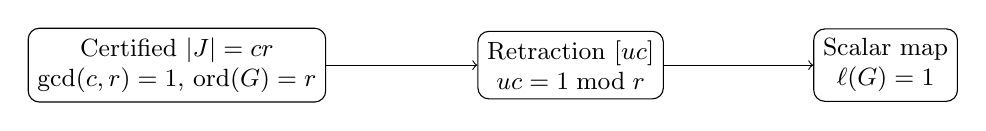
\begin{tikzpicture}[every node/.style={draw,rounded corners,align=center,font=\small}]
\node (a) at (0,0) {Certified $|J|=cr$\\$\gcd(c,r)=1$, $\operatorname{ord}(G)=r$};
\node (b) at (5,0) {Retraction $[uc]$\\$uc=1\bmod r$};
\node (c) at (9,0) {Scalar map\\$\ell(G)=1$};
\draw[->] (a)--(b);\draw[->] (b)--(c);
\end{tikzpicture}\end{center}
\section*{Two boundary examples}
In $J=\mathbb Z/49\mathbb Z$, $r=c=7$, $G=7$ has order seven. Every $X$ passes $[7]([7]X)=0$, but every map to $\mathbf F_7$ kills $G$. Even exhaustive torsion checks cannot prove normalization. In contrast, $J=\mathbf F_7^2$, $G=(1,0)$ admits $\ell(x,y)=x$ although its cofactor is seven. Coprimality is sufficient, not necessary. These are abstract derivations, not cohort curve results.
\section*{Source binding and next check}
At source \texttt{a34ce033054a}, \texttt{native\_solver.rs:1188--1280} checks prime $r$, cofactor arithmetic, source-generator nonzeroness and $r$-torsion of its transfer. It checks projected torsion for sixteen rational points; its README already calls this diagnostic. That excerpt has no explicit nonzero-transfer or coprime-cofactor assertion. Lines 1311--1359 verify $D+\sum Q_i=0$; lines 471--515 store signed coefficients and augmented columns $(b,-a)$.

With additive transfer, $H=[k]P$, $G=\tau(P)$ and a normalized $\ell$, this identity gives $\sum\ell(Q_i)+bk=-a$. The point-class negation identity supplies the signs; order-two classes vanish for odd $r$. Bind destination cardinality, transfer additivity/nonzeroness and retained point semantics next. The complete report gives exact obligations and hashes. No scientific workload or timing was run; cost ratio remains null.
\section*{Sources and status}
Standard group facts: Mathlib \href{https://leanprover-community.github.io/mathlib4_docs/Mathlib/GroupTheory/OrderOfElement.html}{OrderOfElement} (subgroup index and cardinality annihilation), and \href{https://leanprover-community.github.io/mathlib4_docs/Mathlib/LinearAlgebra/Basis/VectorSpace.html}{basis extension}. Background: \href{https://kazutomatsuo.github.io/publications/pdf/e89-a_5_1246.pdf}{Arita et al., IEICE 2006, p.1252}, explicit Scholten pullback example. Original Scholten PDF inaccessible; ePrint endpoint returned 403. No novelty claim. This derivation is not yet kernel-checked or independently reviewed. Review agents remain usage-limited. The expired campaign envelope is unchanged.
\end{document}
